\subsection{Análise do tamanho dos documentos}

É preciso entender entre os documentos que estamos trabalhando o tamanho dos documentos em tokens principalmente porque documentos 
muito pequenos podem não ser recomendados para algoritmos com limitação em \textit{corpus} de dados com documentos pequenos. 
O algoritmo LDA, por exemplo, utilizado para encontrar tópicos em documentos, não tem boa performance com documentos pequenos 
(em documentação encontrada na internet recomenda-se documentos acima de 30 ou 40 tokens).

\subsubsection{Distribuição de tamanhos de documentos}

Para melhor compreender o tamanho dos documentos no meu conjunto de textos eu resolvi usar uma histograma para exibir a distribuição de 
tamanhos dos documentos após executar a limpeza básica de tokens (remoção de tags html e stopwords da linguagem portuguesa). 
O gráfico a seguir mostra esta distribuicão.

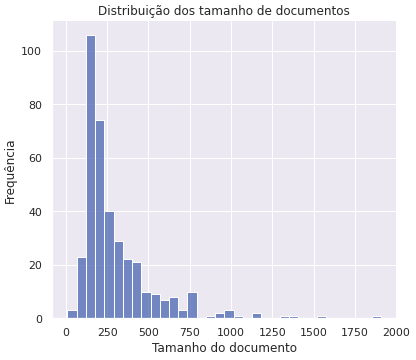
\includegraphics[scale=0.75]{explore/resources/tamanho_documentos.png}

Notei que a maioria dos documentos se concentra em uma faixa de até 750 tokens, então resolvi limitar minha visualização gráfica do eixo 
x a este valor. Pode-se perceber pelo gráfico abaixo que a faixa de maior concentração de documentos é entre 150 e 200 tokens, 
o que é um tamanho bom para o algoritmo que escolhemos. Nota-se também que uma quantidade pequena de documentos se encontra abaixo de 50
tokens, o que também é muito bom. Mais adiante veremos uma distribuição estatística para validar este intervalo.

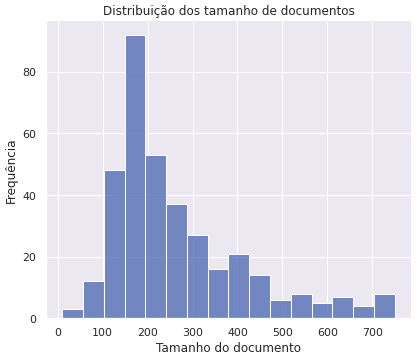
\includegraphics[scale=0.75]{explore/resources/tamanho_documentos_max750.png}

Uma ideia que tive ao longo do desenvolvimento deste projeto foi remover do meu dicionário de treinamento algumas palavras que apareciam
com frequência e que não agregavam nada à comparação dos documentos. Após verificar a frequência eu também achei interessante poder remover 
os verbos do conjunto. Sendo assim eu fiz uma análise do tamanho dos documentos excluindo estes dois conjuntos de palavras. No gráfico 
abaixo é exibida a distribuição dos tamanhos dos documentos após excluir verbos e \textit{stopwords} específicas. O limite de 400
tokens no eixo x foi usado para detalhar melhor a visualização.

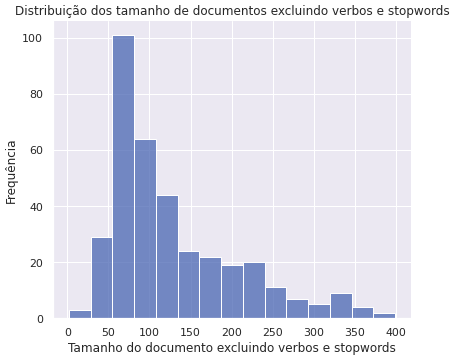
\includegraphics[scale=0.75]{explore/resources/tamanho_documentos_nao_verbo_sw_max400.png}

Mesmo limitando o conjunto anterior a 400 tokens dá pra perceber que há uma faixa de cerca de 30 documentos com tamanho entre 25 
e 50 tokens e achei melhor detalhar mais. Coloquei um limite em 42 para ver graficamente as faixas de tamanhos abaixo dessa linha.
Analisando visualmente percebe-se que 12 documentos estão abaixo deste valor, o que é muito pouco perto do total de 378 documentos 
que restaram no conjunto de posts do blog após a limpeza de posts explicada no processamento de dados.

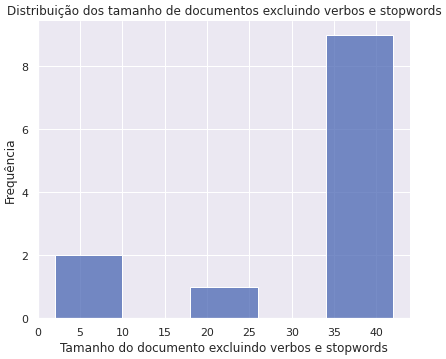
\includegraphics[scale=0.75]{explore/resources/tamanho_documentos_nao_verbo_sw_max42.png}

Para ilustrar um pouco mais esta questão da distribuição dos tamanhos dos documentos eu resolvi criar um gráfico com a comparação entre 
o comportamento dos tamanhos dos documentos originais e o tamanho dos documentos após a remoção de verbos e palavras específicas. Novamente
coloquei limite no tamanho dos documentos para melhor visualização da área mais concentrada.

A imagem a seguir nos mostra ao mesmo tempo que antes os tamanhos dos documentos originais se concentrava entre 150 e 200 tokens e após
a remoção dos dois conjuntos de dados esta faixa de maior concentração passou para entre 50 e 100.

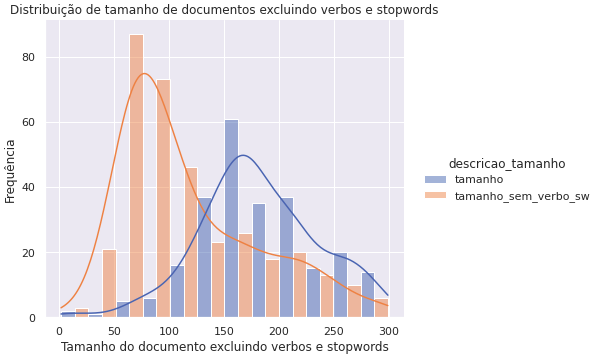
\includegraphics[scale=0.75]{explore/resources/comparacao_distribuicao_tamanhos_kde.png}

Outra forma interessante de ver a relação entre os tamanhos dos documentos antes e após a remoção dos conjuntos de dados é utilizar 
um mapa de calor como este a seguir. As cores mais fortes indicam que maioria dos documentos tinha tamanho entre 150 e 175 antes da remoção
e passou a ter tamanhos entre 65 e 75 sem os verbos e \textit{stopwords} específicas.

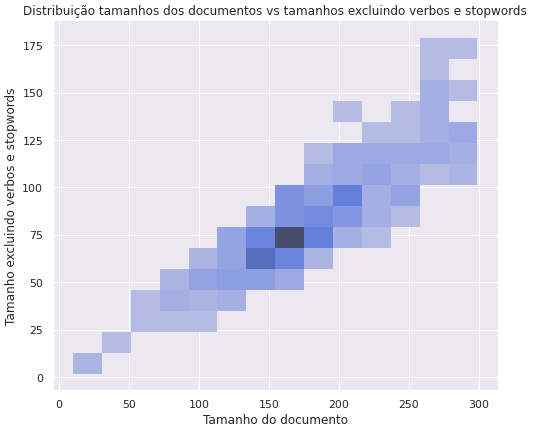
\includegraphics[scale=0.6]{explore/resources/tamanho_documentos_heatmap.png}

\subsubsection{Análise estatística dos tamanhos dos documentos}

Uma outra forma de entender a distribuição dos tamanhos dos documentos é uma descrição estatística. Abaixo está uma tabela 
com várias métricas relacionadas a estes tamanhos, como média, desvio padrão, valor mínimo, valor máximo e percentis diversos.
Optei por incluir, 5\%, 10\%, 90\% e 95\% nos percentis para ver como os tamanhos se comportam para minorias e maiorias.

Após a remoção a média do tamanho de documentos ficou em cerca de 145 tokens e o percentil de 5\% em 49 nos mostra que ainda 
assim a maioria dos documentos está com tamanho aceitável.

\begin{center}
    \begin{tabular}{ |c|c|c| }
        \hline
        Métrica & Documento Original & Documento sem verbos ou \textit{stopwords} específicas \\
        \hline
        count & 378.000000 & 378.000000 \\
        \hline
        mean & 303.706349 & 145.137566 \\
        \hline
        std & 234.920633 & 118.516928 \\
        \hline
        min & 10.000000 & 2.000000 \\
        \hline
        5\% & 111.700000 & 49.000000 \\
        \hline
        10\% & 133.000000 & 57.700000 \\
        \hline
        25\% & 165.000000 & 73.000000 \\
        \hline
        50\% & 216.000000 & 101.000000 \\
        \hline
        75\% & 367.000000 & 179.000000 \\
        \hline
        90\% & 589.200000 & 276.600000 \\
        \hline
        95\% & 747.450000 & 349.600000 \\
        \hline
        max & 1909.000000 & 1033.000000 \\       
        \hline
    \end{tabular}
\end{center}